%!TEX root = ../AST208-notes.tex

\section{Warmup: the simple harmonic oscillator}

Let's begin with a simple system: a mass $m$ attached to a spring with force constant $k$. We'll neglect any dissipation (friction), and then add a driving oscillatory force. In reading these notes, don't dwell so much on the mathematical details; instead try to focus on the gross behavior of the solutions.

\subsection{With no driving force}

\begin{marginfigure}
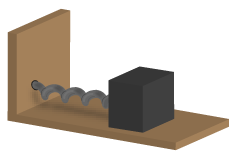
\includegraphics[width=\linewidth]{simple-spring}
\caption[A simple harmonic oscillator]{A simple harmonic oscillator: a mass $m$ on a frictionless surface attached to a  spring with force $F = -kx$.
\label{f.simple-spring}}
\end{marginfigure}

If we put the origin of our coordinate system where the mass is at rest with the spring relaxed, then the equation of motion of the mass is
\begin{equation}\label{e.SHO-basic}
	\DDtt{x} + \frac{k}{m} x = 0.
\end{equation}
You have solved this before: the most general solution is
\begin{equation}\label{e.SHO-general-solution}
	x(t) = x_{0}\cos(\wot) + \frac{v_{0}}{\omega_{0}}\sin(\wot)
\end{equation}
with $\omega_{0}^{2} = k/m$ and with $x_{0}$ and $v_{0}$ being the initial position and velocity of the mass.

\begin{exercisebox}[Solutions to equations for a simple harmonic oscillator]
Verify that equation (\ref{e.SHO-general-solution}) is a solution to equation (\ref{e.SHO-basic}) with initial conditions $\left.x\right|_{t=0}=x_{0}$, $\left.\dif x/\dif t\right|_{t=0} = v_{0}$.
\end{exercisebox}

\subsection{With driving at frequency $\omega \neq \omega_{0}$}

Now let us push on our mass with an oscillating force, $F\cos(\omega t)$ with $\omega\neq\omega_{0}$. A real world example would be holding a vibrating tuning fork near one tuned to a different frequency.  The equation of motion is now
\begin{equation}\label{e.SHO-driven}
	\DDtt{x} + \omega_{0}^{2}x = \frac{F}{m}\cos(\wt).
\end{equation}
You can verify by substitution that a general solution is
\[
	x(t) = \frac{F/m}{(\omega_{0}^{2}-\omega^{2})}\cos(\wt) + A\cos(\wot)+B\sin(\wot).
\]
Let's start with our harmonic oscillator at rest ($v_{0} = \left.\dif x/\dif t\right|_{t=0} = 0$) and at $\left. x\right|_{t=0} = 0$.  With these conditions, we can determine the constants $A$ and $B$; the solution is
\[
	x(t) = \frac{F/m}{(\omega_{0}^{2}-\omega^{2})}\left[\cos(\wt)-\cos(\wot)\right].
\]
Let's recast this by defining $\Delta = \omega_{0} - \omega$, $\omega_{m} = (\omega_{0}+\omega)/2$.  Then
\begin{eqnarray*}
  \omega_{0}^{2}-\omega^{2} &=& (\omega_{0}-\omega)(\omega_{0}+\omega) = 2\Delta\omega_{m},\\
  \cos(\wot) &=& \cos\left(\wmt+\Delta t/2\right) = \cos(\wmt)\cos(\Delta t/2) - \sin(\wmt)\sin(\Delta t/2),\\
  \cos(\wt) &=& \cos\left(\wmt-\Delta t/2\right) = \cos(\wmt)\cos(\Delta t/2) + \sin(\wmt)\sin(\Delta t/2);
\end{eqnarray*}
and we write the solution as
\begin{equation}\label{e.beats}
	x(t) = \left[\frac{F/m}{\Delta\omega_{m}}\sin(\Delta t/2)\right]\sin(\wmt).
\end{equation}
This illustrates the phenomena of \textbf{beats}: the oscillation consists of a carrier signal at frequency $\omega_{m}$ with the amplitude modulated at the slower frequency $\Delta /2$.  Notice that the amplitude increases as $\Delta \to0$, i.e., $\omega\to\omega_{0}$.

\begin{figure*}[hbt]
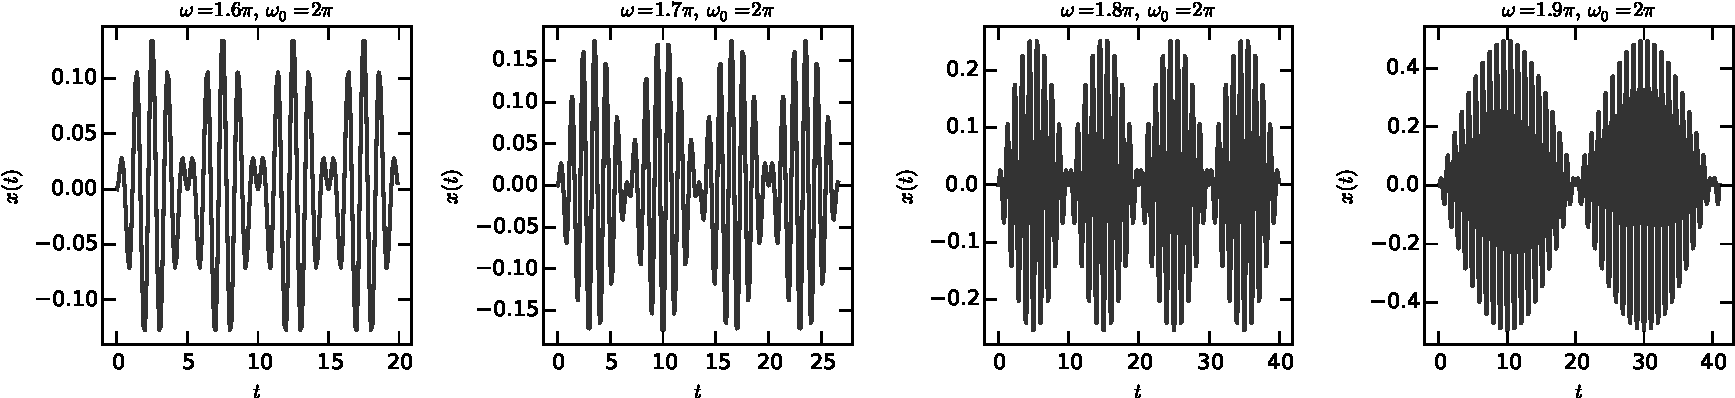
\includegraphics[width=\linewidth]{beats}
\caption[Illustration of beats for four different frequencies]{Illustration of beats for four different frequencies $\omega$.  Notice how the amplitude increases as $\Delta$ becomes smaller.
\label{f.beats}}
\end{figure*}

\subsection{With driving at frequency $\omega_{0}$}

As we saw in the previous example, the amplitude of the driven oscillation increases as $\omega\to\omega_{0}$.  Now let's drive the oscillator precisely at its natural frequency $\omega_{0}$.  The equation of motion is
\begin{equation}\label{e.driven-at-resonance}
	\DDtt{x} + \omega_{0}^{2}x = \frac{F}{m}\cos(\omega_{0}t).
\end{equation}
The general solution is
\[
	x(t) = \frac{Ft}{2m\omega_{0}}\sin(\wot) + A\cos(\wot) + B\sin(\wot).
\]
Notice that the response to the driving grows linearly in time. Suppose our mass has been oscillating with no driving, and at $t=0$ we turn on $F$.  Suppose further that at time $t=0$ the position of the mass is $0$ and the velocity of the mass is $v_{0}$.  Then our solution is
\begin{equation}\label{e.resonant-oscillator}
	x(t) = \left[\frac{Ft}{2m\omega_{0}} + \frac{v_{0}}{\omega_{0}}\right]\sin(\wot).
\end{equation}

\begin{exercisebox}[Solutions to equations for a driven oscillator]
Verify that equation~(\ref{e.resonant-oscillator}) is a solution to equation~(\ref{e.driven-at-resonance}).  For the resonant oscillation in eq.~(\ref{e.resonant-oscillator}), what is the time for the amplitude to double?
\end{exercisebox}

\newthought{In reality, other effects may eventually limit the amplitude's growth.} The spring may snap when stretched too far. The wine glass may shatter when the singer hits a high note. Nevertheless, when a driving term oscillates near a natural frequency in the system, the result is for the oscillation amplitude to grow.
\section{The damped, driven oscillator}

For completeness, let's make our model even more realistic by adding some \textbf{damping}.  We add a friction or drag force that is proportional to velocity, $F_{\mathrm{friction}} = -\Gamma \dif x/\dif t$. Our complete equation of motion is then
\begin{equation}
	\DDtt{x} + \frac{\Gamma}{m} \DDt{x} + \omega_{0}^{2}x = \frac{F}{m}\cos(\omega t).
\end{equation}
The solution to this is more complicated than the previous examples, but it is found using the same technique.  The general solution for initial conditions $\left.x\right|_{t=0} = x_{0}$ and $\left.\dif x/\dif t\right|_{t=0} = v_{0}$ is
\begin{eqnarray}
\label{e.general-solution-ddo}
x(t) &=& \frac{F\womw/m}{\womw^{2}+\gw}\cos(\omega t) \\
	&& + \frac{\Gamma\omega F/m^{2}}{\womw^{2}+\gw}\sin(\omega t)\nonumber \\
	&& + \left[x_{0}-\frac{F\womw/m}{\womw^{2}+\gw}\right]e^{-\Gamma t/2m} \cos(\omega_{\Gamma}t) \nonumber\\
	&& + \left[\frac{v_{0}}{\omega_{\Gamma}}-\frac{\Gamma\omega F/m^{2}}{\womw^{2}+\gw}
	\,\frac{\omega}{\omega_{\Gamma}}\right]e^{-\Gamma t/2m} \sin(\omega_{\Gamma}t), 
	\nonumber
\end{eqnarray}
with
\[ \omega_{\Gamma} = \omega_{0}\left(1-\frac{(\Gamma/m)^{2}}{4\omega_{0}^{2}}\right)^{1/2}. \]
This formula is long, so let's look at limiting cases.  First, suppose we turn off the driving force by setting $F\to 0$. Also, let's set $v_{0}\to0$ as well. Then
\[
	x(t) = x_{0}e^{-\Gamma t/2m} \cos\left(\omega_{\Gamma}t\right).
\]
This is similar to our simple example, but the frequency is slightly shifted from $\omega_{0}$ to $\omega_{\Gamma}$,
and the amplitude decays as $e^{-\Gamma t/2m}$. A plot is shown in Figure~\ref{f.damped}.

\begin{figure*}[ht]
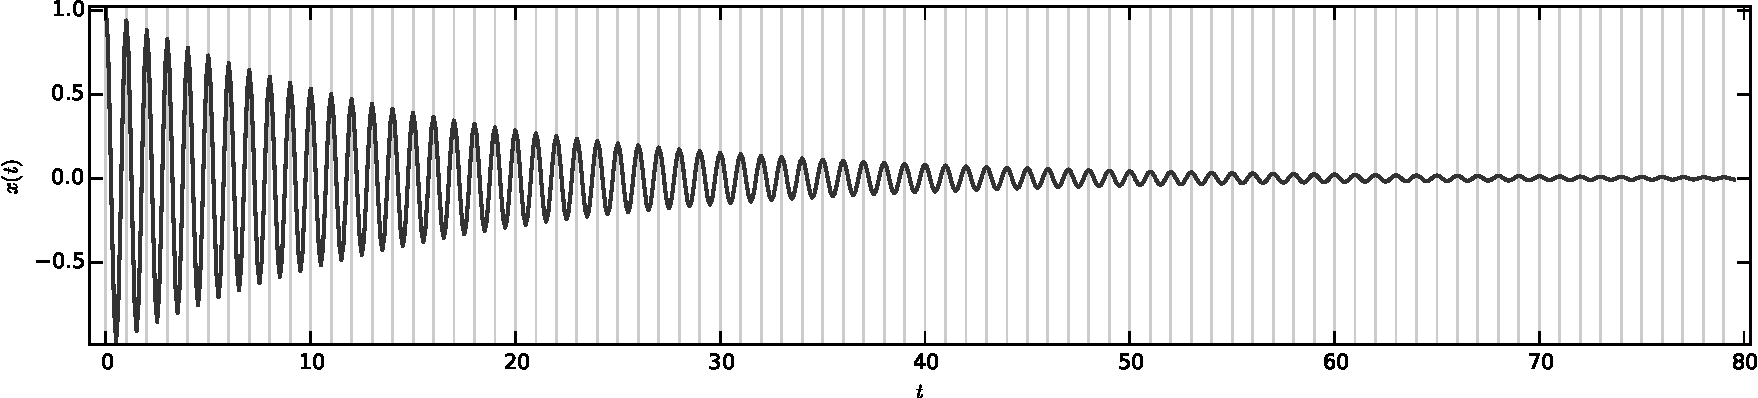
\includegraphics[width=\linewidth]{damped}
\caption[A damped oscillator]{A damped oscillator, with frequency $\omega_{0} = 2\pi$ and damping constant $\Gamma/m = 0.04\pi$. The light gray vertical lines indicate the period $2\pi/\omega_{0}$.
\label{f.damped}}
\end{figure*}

Now if we turn on our driving force $F$ and set $\Gamma\to0$, then we recover equation~(\ref{e.beats}), as expected. So, for the general case, we expect that the oscillation will look like that in Figure~\ref{f.beats} at early times. After a time $2m/\Gamma$, however, the last two terms of equation (\ref{e.general-solution-ddo}) will decay and there will only be the first two terms, which oscillate at frequency $\omega$.  Figure~\ref{f.damped-driven} shows the solution in this case.  The light gray vertical lines mark off periods $2\pi/\omega_{0}$; you can see that as the beats disappear the frequency shifts from approximately $\omega_{0}$ to $\omega$.

\begin{figure*}[ht]
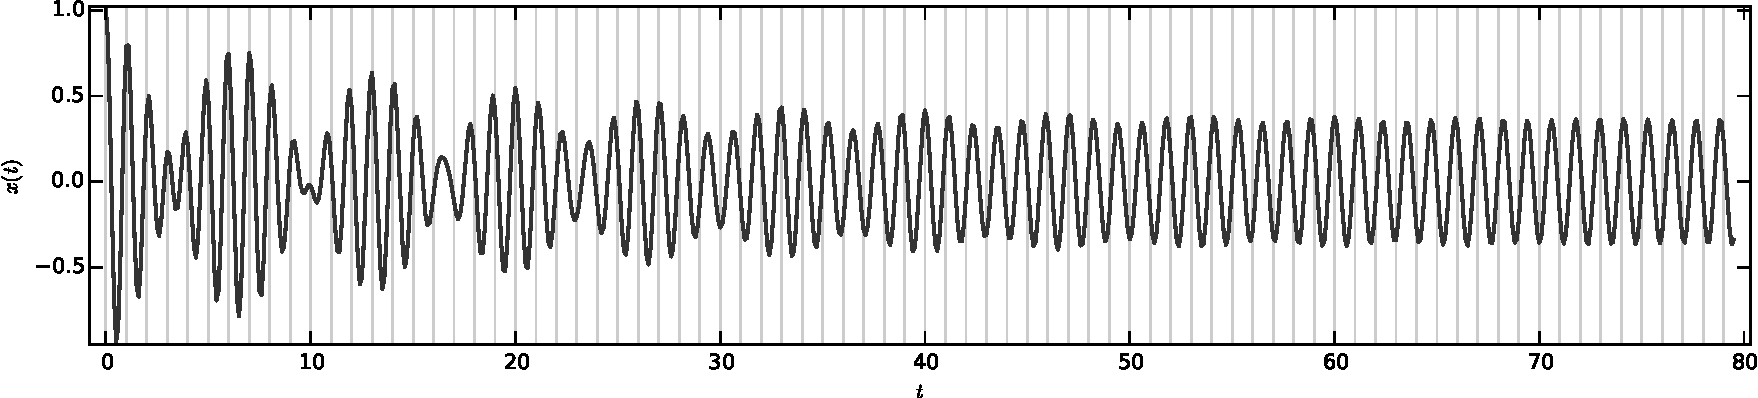
\includegraphics[width=\linewidth]{damped-driven}
\caption[A damped, driven oscillator]{A damped, driven oscillator, with frequency $\omega_{0} = 2\pi$, damping constant $\Gamma/m = 0.04\pi$, and driving force $4.0/m\,\cos(\omega t)$ with $\omega=1.7\pi$. The light gray vertical lines indicate the period $2\pi/\omega_{0}$.
\label{f.damped-driven}}
\end{figure*}

In the limit $\omega \to \omega_{0}$ the solution goes to 
\[ x(t) = \frac{F}{\Gamma\omega_{0}} \sin(\omega_{0} t).\]
For the parameters used to make Figure~\ref{f.damped-driven}, this amplitude is $F/(\Gamma\omega_{0}) = 5.1$; the final oscillation amplitude for the case shown in the plot is much less than this because the driving frequency is $\omega = 0.85\omega_{0}$.

\section{Applications to the solar system}
Planets, moons, and other minor bodies in solar system have made millions to billions of orbits. As the previous section demonstrates, even a small perturbing force, if applied near a natural frequency of a system, can eventually produce a large response when applied over such a long dynamical time. 

There are many bodies in the solar system that are locked into a stable resonance. For example, Pluto is locked into a stable 2:3 resonance with Neptune (that is, Pluto completes 2 orbits for every 3 of Neptune), and the Jovian moons Io, Europa, and Ganymede are locked into a 1:2:4 resonance. Resonances can also lead to instability, in which a body's orbit is distorted to the point that it crosses the orbit of another planet, at which point that body either collides with the other planet or is scattered out of the solar system.  For example, the Kirkwood gap in the asteroid belt is located at the 3:1 resonance with Jupiter (see Fig.~2.10 of \citetalt{Lissauer2013Fundamental-Pla}). Numerical calculations find that the precession of Mercury's perihelion is coming into resonance with that of Jupiter, leading to a 1\% chance over the next \val{5}{\Giga\yr} of Mercury colliding with the Sun or Venus, and a smaller possibility of the entire inner solar system becoming unstable\cite{Laskar2009Existence-of-co} over that time.

\newthought{Torques exerted on a planet's equatorial bulge} by other solar system bodies can cause that planet's obliquity to vary.  Saturn's large (relative to Jupiter) axial tilt is thought to be caused by a spin-orbit resonance between the precession of Saturn's axis the precession of Neptune's orbital plane\cite{Ward2004Tilting-Saturn.}.  Mars's axial tilt wanders considerably over a few Myr timescale and has reached tilts as large as $60^{\circ}$ in the past.  The large moment of inertia of the Earth-Moon system keeps Earth's axial tilt from wandering to such extreme values; nevertheless, the Earth's inclination does oscillate by $<1^{\circ}$ on a $\val{40\,000}{\yr}$ timescale.  This wandering of the inclination, along with variations in the orbital eccentricity, are thought to explain the quasi-periodic ice ages on Earth over the last few million years\cite{Zachos2001Trends-Rhythms-}.

